%\section{New technique or technique adaptation}
\section{Alinhamento Semi-automático}
\label{sec:technique}

Para inserir um detalhe $\mathcal{D}$ em $\mathcal{S}$, é necessário inicialmente a intervenção do usuário para determinar em que região da superfície $\mathcal{S}$ o detalhe $\mathcal{D}$ deve ser inserido, e qual sua orientação. Desse modo, precisamos encontrar uma transformação $T$ que alinhe $\deta$ em $\super$. Em nosso trabalho, optamos por limitar estas transformações apenas a movimentos rígidos.

Para tornar nossa interface mais simples e amigável para o usuário, realizamos o alinhamento baseado em correspondências do tipo $c_i = (s_i, d_i), s_i \in \mathcal{S}, d_i \in \mathcal{D}$ fornecidas pelo usuário, como ilustra a FIGURA!!!!! Dado um conjunto de correspondências $C=\left\{c_1,\dots\,c_n\right\}$, existem diversas abordagens para encontrar um movimento rígido $T$ que minimize a distância entre as correspondências. Alguns desses métodos usam, além geometria das correspondências, os seus vetores normais. Porém, para o nosso problema, os vetores normais não devem ser necessariamente iguais nas correspondências, visto que são provenientes de geometrias distintas. Desse modo, optamos por usar o método de Horn \cite{horn:1987}, que se baseia apenas na minimização da distância entre a posição geométrica dos pontos correspondentes, ou seja, buscamos uma rotação $R$ e uma translação $t$ que minimizem
\begin{equation}
\sum_{i=1}^n \|s_i - Rd_i - t \|.
\end{equation}
A solução deste problema de minimização baseada no uso de quatérnios unitários pode ser encontrada em \cite{horn:1987}. Destacamos que, apesar de calcular uma rotação $R$ e uma translação $t$, apenas a rotação $R$ será usada no restante do nosso método, visto que a reconstrução baseada em gradientes discretos é invariante por translações.


%\begin{figure}[h]
%\center
%    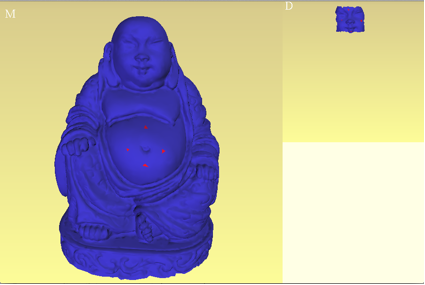
\includegraphics[width=8cm]{ImagemICP2}
%        \label{ICP}
%\end{figure}
%\vspace{4mm}
\subimages[htb]{Iterative Closest Point}{ICP}{
  \subimage{.7}{ImagemICP2}%
}


%
%Our technique aims at obtaining that result. It particularly suits to the problem since it is formulated as\ldots{}


%%------------------------------------------------------------------------- 
%\subsection{Formulation}
%
%
%%------------------------------------------------------------------------- 
%\subsection{Solution}
%
%
%%------------------------------------------------------------------------- 
%\subsection{Initialization and tuning}